\documentclass[10pt]{article}
\usepackage[letterpaper,margin=0.725in]{geometry}

\usepackage{fancyhdr}
\usepackage{amsmath}
\usepackage{mathtools}
\usepackage{hyperref}
\usepackage[english]{babel}
\usepackage{graphicx}
\usepackage{float}
\usepackage{caption}
\usepackage{amssymb}
\usepackage{caption}
\usepackage{amstext} % for \text macro
\usepackage{array}   % for \newcolumntype macro
\allowdisplaybreaks

\usepackage[T1]{fontenc}
\usepackage[numbered,framed]{matlab-prettifier}

\hypersetup{ colorlinks=true, linkcolor=blue}

\DeclareMathOperator{\atantwo}{atan2}
\newcolumntype{C}{>{$}c<{$}} % math-mode version of "l" column type

\pagestyle{fancy}
\lhead{RBE 500 - PA \#2 \newline Team 2: Peter Campellone, Aislin Hanscom, Christopher Poole}
\rhead{Due: 7/13/2021}

\begin{document}

\setlength{\abovedisplayskip}{6pt}
\setlength{\belowdisplayskip}{3pt}
\setlength{\abovedisplayshortskip}{4pt}
\setlength{\belowdisplayshortskip}{4pt}

\textbf{Package overview:}
\begin{itemize}
	\item Inside \texttt{catkin\_ws/src}, the main package is \texttt{scara\_robot}. It does not directly contain any nodes or launch files, but is a way to organize all of the other nodes.
	\begin{itemize}
		\item New package:
		\begin{itemize}
			\item The \texttt{scara\_pd\_controller} package implements a proportional and derivative controller for joint 3 (prismatic joint). The controller functions by reading the current joint position using the \\ \texttt{gazebo/get\_joint\_properties} service, calculating the necessary input into the joint, and applying the input force using the \texttt{gazebo/apply\_joint\_effort} service.
		\end{itemize}
		
		\item Old packages used (from PA \#1):
		\begin{itemize}
			\item The \texttt{scara\_gazebo} package includes the launch files for the gazebo world.
			\item The \texttt{scara\_description} package includes the URDF files for the robot as well as the rviz launch files.
		\end{itemize}
	\end{itemize}
\end{itemize}

\begin{enumerate}
	\item Fix all of the joints except the last joint by changing the joint type field of the corresponding joints to "fixed" in the robot description file.
	
	The following changes were made to the XACRO file:
	
	...
	
	...
	
	\item Write a position controller node.
	
	\begin{itemize}
		\item Get positions from Gazebo and be able to send joint efforts.
		
		\item Design PD controller (tune gains, don't calculate)
		
		\item Implement service that takes in a reference (desired) position for the last joint.
		
		\item Record both the reference position and current position in a text file. Plot the comparison in MATLAB.
		
	\end{itemize}

	The E.O.M. of our third link for our controller is below:
	
	\begin{minipage}[h]{0.3\textwidth}
		\centering
		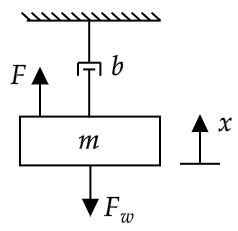
\includegraphics[width=0.7\textwidth]{figures/mass_damper.png}
	\end{minipage}
	\begin{minipage}[h]{0.5\textwidth}
		\begin{align*}
			&\sum{F} = m a \Rightarrow F - b \dot{x} - F_w = m \ddot{x} \\
			&m \ddot{x} + b \dot{x} + F_w = F \\
			&H(s) = \frac{X(s)}{F(s)} = \frac{1}{m s^2 + b s + F_w}
		\end{align*}
	\end{minipage}
	
	Our controller (PD) will have the following form:
	\begin{align*}
		C(s) = k_p + k_d s \Rightarrow c(t) = k_p E + k_d \frac{dE}{dt}
	\end{align*}
	
	where $E = d_{3,\text{desired}} - d_{3,\text{current}}$ and $dt$ is the time step of the controller loop. $k_p$ and $k_d$ are the gains for the proportional and derivative terms, respectively.
	\\
	
	The main file for the controller exists in the \texttt{scara\_pd\_controller} package under the \texttt{pd\_control.py} file.
	\\
	
	The control values are calculated within the \texttt{pd\_control} function:
	
\begin{lstlisting}[style=Matlab-editor,basicstyle=\mlttfamily,escapechar=`]
def pd_control(joint, pos_cur, pos_des, kp, kd):
	global E_old
	
	E = pos_des - pos_cur
	d_err = (E - E_old)/(1/rate)
	f = -(kp*E + kd*d_err)
	
	if debug == True:
		print("\nerr = %f,  d_err = %f" % (E, d_err))
		print("\npos_des = %f, pos_cur = %f" % (pos_des, pos_cur))
		print("\nSending joint force f = [%f]" % (f)) # printing calculated values to terminal
	
	je_service = rospy.ServiceProxy('/gazebo/apply_joint_effort', ApplyJointEffort)
	zero_time = rospy.Time()
	tick = rospy.Duration(0, int((1/rate)*10**9))
	je_service(joint, f, zero_time, tick)
	
	if print_to_file == True:
		file1.write("%f,%f,%f,%f\n" % (pos_cur, pos_des,f,1/rate))
	
	E_old = E 
	
	return f
\end{lstlisting} 

	The joint positions are obtained in the following function:
	
\begin{lstlisting}[style=Matlab-editor,basicstyle=\mlttfamily,escapechar=`]
def request_joint_status(joint):
	global d3
	global d3_old
	
	joint_stauts = rospy.ServiceProxy('/gazebo/get_joint_properties', GetJointProperties)
	resp = joint_stauts(joint)
	
	d3 = -resp.position[0]
	
	if debug == True:
		print("\n\nReceived joint position: [%f] (d3) (meters)" % (d3)) # printing received data to terminal
	
	pd_control('joint5', d3, d3_des, kp, kd)
	
	return resp
\end{lstlisting} 

	The reference position is set with the following function
	
\begin{lstlisting}[style=Matlab-editor,basicstyle=\mlttfamily,escapechar=`]
def service_handle(data):
	global d3_des
	
	d3_des = data.d3_des
	
	if debug == True:
		print("\nReceived reference position d3 = %f]" % (d3_des)) # printing converted values to terminal
	
	if d3_des >= 0 or d3_des <=1:
		success = True
	else:
		success = False
	
	return success
\end{lstlisting} 

	Steps to run:
	
	\begin{enumerate}
		\item \texttt{catkin\_make}
		\item \texttt{source devel/setup.bash}
		\item \texttt{roslaunch scara\_gazebo scara\_world.launch}
		\item In a new window, \texttt{rosrun scara\_pd\_controller pd\_control.py}. The controller will begin controlling the joint to its home position ($d_3 = 0$).
		\item In a new window, \texttt{rosservice call /scara/JointControlReference "d3\_des: X.XX"} where X.XX is any number between 0 and 1 (joint limits).
	\end{enumerate}


	The results from MATALB are shown below from setting the reference position to $0.5$, $0.75$, then $0.25$:

	\begin{figure}[H]
		\centering
		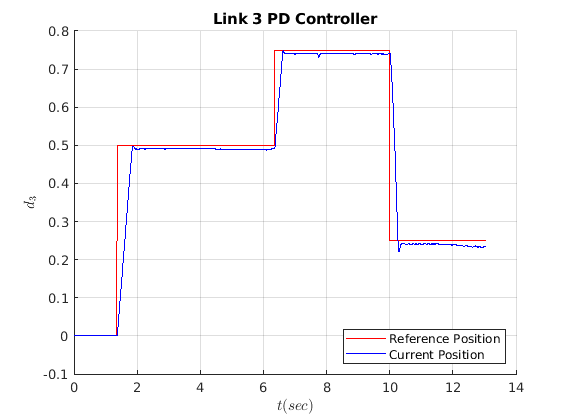
\includegraphics[width=0.75\textwidth]{figures/link_3_pd_plot1.png}
	\end{figure}
	
	From the above plot, we can see that the position of the link is approaching the reference position with limited overshoot (due to the tuning of the derivative term). There is a slight steady-state error due to the absence of an integral term. The addition of an integral term would accumulate that steady-state error and bring the current link position closer to the reference. 
	\\
	
	The resulting gains are below:
	\begin{align*}
		k_p = 1100 \hspace{0.5cm} k_d = 35
	\end{align*}
	
	These gains were determined experimentally by observing the overshoot and reaction of the link.
	\\
	
	To show the effect of having the derivative term in our controller, we can also show the link's response with a proportional only controller ($k_d = 0$):
	
	\begin{figure}[H]
		\centering
		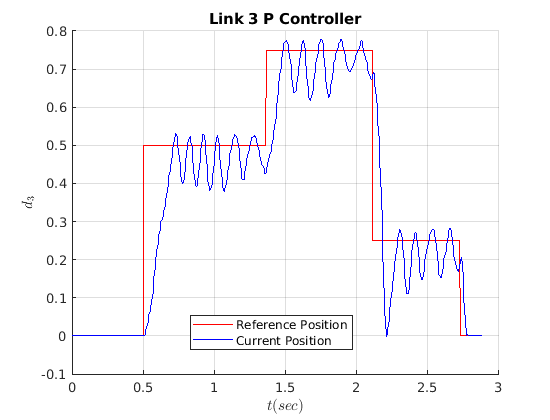
\includegraphics[width=0.75\textwidth]{figures/link_3_p_plot1.png}
	\end{figure}

	It is apparent that there is a large amount of oscillations about the reference positions. The derivative term helps dampen this greatly.

\end{enumerate}
\end{document}



